\scanpage{40}
% archive foliation: 39
\deleted{\unsure{Preuve}} Pour le prouver, on peut supposer $S$, $Y$, les $X_i$, \inserted{$T$} affines d'anneaux $A$, $B$, $B_i$, $A'$, \inserted{les} $F_i$ définis par \deleted{$M_i$} un $B_i$-module $M_i$. Soit $L^{(i)}$ une résolution libre de $M_i$ comme $B_i$-module, posons
\[
K=\mathop{\bigotimes}\limits_{1\leq i\leq n}{}_{B}L^{(i)}
\]
Alors \deleted{pour tout $i$}, les $L^{(i)}$ sont \uline{plats sur $A$}, et comme $M_i$ est plat sur $A$, il en s'ensuit que $L'^{(i)}_{\deleted{\unsure{A'}}}=L^{(i)}\otimes_A A'$ est une résolution de $M'_i=M_i\otimes_A A'$, évidemment $B'_i$-libre (où $B'_i=B_i\otimes_A A'$).

Donc la cohomologie de
\[
K'=K\otimes_A A'\deleted{\unsure{\otimes_B B'}}\inserted{{}=K\otimes_B B'}=\mathop{\bigotimes}\limits_{1\leq i\leq n}{}_{B'}L^{(i)}\otimes_B B'=\mathop{\bigotimes}\limits_{1\leq i\leq n}{}_{B'}L^{(i)'}
\]
n'est autre que $\operatorname{Tor}_{\unsure{\alpha|*}}^{B'}(M'_1,-,M'_n)$. Or comme $K$ est $A$-plat, on a une suite spectrale homologique
\[
H_{*}^{\deleted{*}}(K\otimes_A A')\Longleftarrow\operatorname{Tor}_p^A(H_q(K),A'))
\]
i.e.
\[
\operatorname{Tor}_*^{B'}(M'_1,-,M'_n)\Longleftarrow\operatorname{Tor}_p^A(\operatorname{Tor}_q^B(M_1,-,M_n),A').
\]
Il s'ensuit que si $\operatorname{Tor}_q^B(M_1,-,M_n)$ est $A$-plat pour $q\leq N$, on a l'\deleted{\unsure{établie}} isomorphisme en cause.

\margin{\diagram{$\left.\begin{tikzcd}[row sep=small,column sep=small]
M_1&M_2&\unsure{M'|M'_1}&M'_2\\
B_1&B_2&B'_1&B'_2\\
B&&B'&\\
A&&A'&
\end{tikzcd}\right\}$}}

\margin{\figure{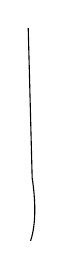
\begin{tikzpicture}\draw (0,0)--(.05,-1.9)..controls (.11,-2.3) and (.08,-2.55)..(.03,-2.7);\end{tikzpicture}}\unsure{au lieu de} la suite spectrale, on peut aussi invoquer un résultat sur la cohomologie d'un complexe.}
